\section{V3}
\subsection{Meiose}

\subsection{Mendelsche Gesetze}

\subsection{Erbgänge / Stammbäume}

\subsection{Gründe für Abweichungen von Mendelschen Erbgängen}

\subsection{Aufgaben zur Übung 3}
\subsubsection{Aufgabe 1}
\textbf{a.)}
\begin{itemize}
	\item Sensitivität: gibt den Anteil der korrekt als positiv klassifizierten Objekte an der Gesamtheit der tatsächlich positiven Objekte an ($\mathbb{P}(P|K)$)
	\item Spezifität: gibt den Anteil der korrekt als negativ klassifizierten Objekte an der Gesamtheit der in Wirklichkeit negativen Objekte an ($\mathbb{P}(\overline{P}|\overline{K})$)
	\item Prävalenz: welcher Anteil der Menschen einer bestimmten Gruppe (Population) definierter Größe zu einem bestimmten Zeitpunkt an einer bestimmten Krankheit erkrankt ist\\
	Prävalenz=Anzahl der zum Untersuchungszeitpunkt Kranken / Anzahl der in die Untersuchung einbezogenen Individuen
\end{itemize}

\underline{Vierfeldertafel}\\
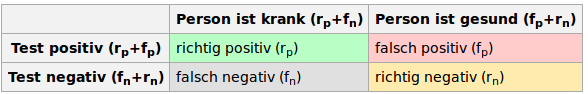
\includegraphics[width=1\textwidth]{lectures/V3/pix/Konfusionsmatrix.png}

\includegraphics[width=0.5\textwidth]{lectures/V3/pix/Binary-classification-file.png}
\newpage
\textbf{b.)}\\
gegeben:
\begin{itemize}
	\item K=\{Patient ist krank\}
	\item P=\{Test ist positiv\}
	\item Sensitivität: $\mathbb{P}(P|K)=0,95$
	\item Spezifität: $\mathbb{P}(\overline{P}|\overline{K})=0,90$
	\item Prävalenz: $\mathbb{P}(K)=0,1$
\end{itemize}

gesucht:\\
\begin{itemize}
	\item positiv prädiktiver Wert (PPW): \\
	$\mathbb{P}(K|P) = \underbrace{\frac{\mathbb{P}(P|K) \cdot \mathbb{P}(K)}{\mathbb{P}(P)}}_{Satz\ von\ Bayes} = \underbrace{\frac{\mathbb{P}(P|K) \cdot \mathbb{P}(K)}{\underbrace{\mathbb{P}(P|\overline{K})}_{=1-\mathbb{P}(\overline{P}|\overline{K})} \cdot \mathbb{P}(\overline{K}) + \mathbb{P}(P|K) \cdot \mathbb{P}(K)}}_{totale\ Wahrscheinlichkeit}$\\
	$\mathbb{P}(K|P) = \frac{0,95 \cdot 0,1}{0,1 \cdot 0,9 + 0,95 \cdot 0,1} = $ \underline{\underline{0,513513514}}
	\item negativ prädiktiver Wert (NPW):\\
	$\mathbb{P}(\overline{K}|\overline{P})= \frac{\mathbb{P}(\overline{P}|\overline{K}) \cdot \mathbb{P}(\overline{K})}{\underbrace{\mathbb{P}(\overline{P})}_{1-\mathbb{P}(P)}} = \frac{\mathbb{P}(\overline{P}|\overline{K}) \cdot \mathbb{P}(\overline{K})}{1 - (\mathbb{P}(P|\overline{K}) \cdot \mathbb{P}(\overline{K}) + \mathbb{P}(P|K) \cdot \mathbb{P}(K))}$\\
	$\mathbb{P}(\overline{K}|\overline{P})= \frac{0,9 \cdot 0,9}{1-(0,1 \cdot 0,9 + 0,95 \cdot 0,1)} =$ \underline{\underline{0,993865031}}
\end{itemize}

\textbf{c.)}
\\
gegeben:
\begin{itemize}
	\item Sensitivität: $\mathbb{P}(P|K)=0,95$
	\item Spezifität: $\mathbb{P}(\overline{P}|\overline{K})=0,90$
	\item Prävalenz: $\mathbb{P}(K)=0,05$
\end{itemize}

gesucht:\\
\begin{itemize}
	\item positiv prädiktiver Wert (PPW)= \underline{\underline{0,$\overline{33}$}}
	\item negativ prädiktiver Wert (NPW)= \underline{\underline{0,997084548104956}}
\end{itemize}

\textbf{d.)}
siehe R-Script

\subsubsection{Aufgabe 2}

\subsubsection{Aufgabe 3}
siehe R-Script